\chapter{Convección Mixta en Flujos Completamente Desarrollado}


La finalidad de este capítulo es que el lector/jurado comprenda la forma de abordar el problema estudiado. Así como las magnitudes y parámetros relevantes del problema. 


\newpage

\section{Casos simulados} 

Los resultados de las simulaciones realizadas en este capítulo corresponden a un flujo completamente desarrollado tanto térmica como hidrodinámicamente. Se utilizaron valores de números adimensionales tales que Re$_o$=2100, 3150, 4278, 5000, Pr=0.071, 0.71 y valores de Richardon en el rango 0.04 $\lesssim$ Ri$_b$ $\lesssim$ 106. En la Figura \ref{fig:map_flow_regime} se expone un ``mapa'' del régimen de flujo donde se gráfica el número de Reynolds\footnote{Número de Reynolds basado en el diámetro hidráulico: $Re^D_b = 8/3 \hspace*{1mm} Re_o$} versus el número de Richardson. De acuerdo al diagrama de Moody \cite{white}:

\begin{itemize}
	\item para valores de Re$^D_b$ $<$ 2000 el régimen es laminar,
	\item si 2000 $\lesssim$ Re$^D_b$ $\lesssim$ 4000 el régimen es de transición,
	\item y si Re$^D_b>$ 4000 el régimen es turbulento.
\end{itemize}
Por otra parte, el fenómeno de convección es \cite{incropera,cengelheat}:

\begin{itemize}
	\item forzado si Ri$_b<$ 0.1,
	\item mixto si 0.1 $<$ Ri$_b$ $<$10,
	\item y natural si Ri$_b$ $>$10.
\end{itemize}

\begin{figure}[H]
  \centering
    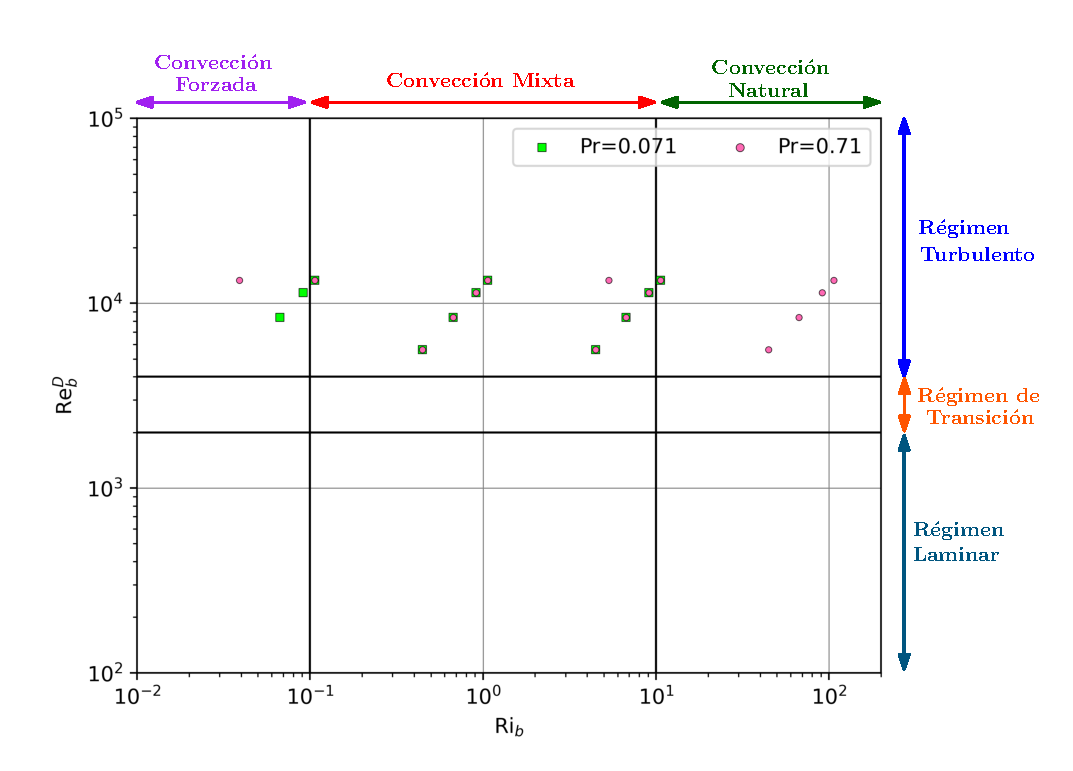
\includegraphics[width=0.7\textwidth]{figures/cap5/map.eps}
  \caption{Mapa de regímenes de los casos simulados.}
  \label{fig:map_flow_regime}
\end{figure}

La totalidad de casos se encuentra en un régimen de flujo turbulento. En su mayoría, los casos se encuentran en flujo de convección mixta, sin embargo, contamos con casos donde predomina la convección forzada, y por otro lado, donde domina la convección natural. Esto brinda un espectro más amplio para el análisis del problema.




\section{Perfil de velocidad y de temperatura}

En esta sección se presentan, a modo de ejemplo, los perfiles de temperatura y velocidad (adimensionales) de los casos con Re$_o$=5000 y Pr=0.71 a fin de comparar el efecto del aumento de la fuerza boyante. Aumentar la fuerza boyante, o el número de Ri$_b$, es equivalente a aumentar el flujo de calor ya que Ri$_b$ $\propto$ $q''_w$. En otras palabras, el aumento de la boyancia en un sistema físico equivale a aumentar la energía térmica que se le entrega a través de las paredes cuando el fluido es ascendente\footnote{También es equivalente a quitarle energía térmica (enfriar las paredes) cuando la dirección del flujo es descendente.} 


\begin{figure}[H]
  \centering
  \subfloat[]{
    \includegraphics[width=0.49\textwidth]{figures/cap5/Re5000-Pr071/phi_mean_profile.png}
    	\label{fig:phi-Re5000-Pr071}}
  \subfloat[]{
    \includegraphics[width=0.49\textwidth]{figures/cap5/Re5000-Pr071/ux_mean_profile.png}
    	\label{fig:ux-Re5000-Pr071}}
  \caption{}
  \label{fig:Re5000-Pr071}
\end{figure}

Cerca de las paredes, la temperatura del fluido es mayor y por tanto es menos denso que el fluido que se encuentra en el seno del canal, y por lo tanto, se produce un gradiente de densidad. Eso se traduce en un aumento de la velocidad (debido fuerza boyante) que eleva verticalmente al fluido calentado cerca la pared y que a su vez arrastra fluido desde la zona central del canal, tal como se observa en la Figura \ref{fig:ux-Re5000-Pr071}. En este último gráfico, es posible distingir, claramente, los tres regímenes de convección. 

En la Figura \ref{fig:phi-Re5000-Pr071} se presenta los perfiles de temperaturas. Los casos se pueden dividir, a priori, en dos grupos: el primer grupo que corresponde a Rib$_b$ de 0.04 a 1.06 y el segundo grupo compuesto por valores de 5.33 a 106.5. En el primer grupo, se produce un aumento de temperatura en el seno del fluido reduciendo la transferencia de calor (como se verá en la sección \ref{sec:nu}). Luego, en el segundo grupo se produce un descento de la temperatura en el seno del fluido mejorando la transferencia de calor. En ese sentido, el sistema es más eficiente para ``evacuar'' el calor suministrado a medida que Ri$_b$ es más alto (o $q''_w$), y por lo tanto, genera una disminución en la temperatura de las paredes. Desde el punto de vista técnico, esto es de utilidad para sistemas de refrigeración. 

Por último, el fluido adyacente a las paredes, como se mencionó antes, al ser más liviano, asciende verticalmente y arrastra fluido desde seno del canal hacia las paredes, lo cuál genera que el fluido se mezcle, se redistribuya la energía, y por tanto, la temperatura a lo largo del canal es más uniforme dando lugar a esa forma más ``achatada'' en el centro.       


\section{Subcapa viscosa y región de ley logarítmica}

Por su parte, la Figura \ref{fig:ux-log-Re5000-Pr071} muestra buen acuerdo con ley lineal  cerca de la pared indicando que, sea cual fuese el régimen de convección, la ley de pared sigue siendo válida en convección mixta y por lo tanto útil para la construcción de modelos de turbulencia [referencia?].   


\begin{figure}[H]
  \centering
  \subfloat[]{
    \includegraphics[width=0.49\textwidth]{figures/cap5/Re5000-Pr071/phi_mean_plus_log_profile.png}
    	\label{fig:plus-phi-log-Re5000-Pr071}}
  \subfloat[]{
    \includegraphics[width=0.49\textwidth]{figures/cap5/Re5000-Pr071/ux_mean_plus_log_profile.png}
    	\label{fig:plus-ux-Re5000-Pr071}}
  \caption{\textcolor{magenta}{Estas gráficas están incompletas, falta cambiar el eje y a escala lineal y agregar la ley logaritmica en ambos casos}}
  \label{fig:Re5000-Pr071}
\end{figure}




\section{UHF vs UWT}

En la sección [REF-VALIDACIONES] se utilizaron las simulaciones obtenidas por Guo y Prasser \cite{guo2022direct} para validar la herramienta numérica utilizada. El sistema estudiado por dichos autores corresponde a una configuración física distinta que al sistema estudiado en este trabajo, sin embargo, resulta útil comparar los perfiles de velocidad y temperatura, para entender en mayor profundidad el fenómeno de convección. En esta sección se pretende cotejar las dos configuraciones físicas establecidas: UHF\footnote{\textit{Uniform Heat Flux}} y UWT\footnote{\textit{Uniform Wall Temperature}}. El primero corresponde a los parámetros Re$_o$=3150, Pr=0.071 y Ri$_b$=0.67, y el segundo, a Re$_o$=3500, Pr=0.025 y Ri$_b$=0.5. Si bien los parámetros involucrados no son idénticos, están en el mismo orden de magnitud, para fines cualitativos, esto es más que adecuado para análizar la física detrás de ellos. Las Figuras \ref{fig:guocomp_ux} y \ref{fig:guocomp_phi} exponen los perfiles de velocidad en la dirección de la corriente y la temperatura de ambas configuraciones, respectivamente. En ambos casos se normaliza los perfiles con el máximo de la propia curva.  

\begin{figure}[H]
  \centering
  \subfloat[]{
    \includegraphics[width=0.49\textwidth]{figures/cap5/phi_mean_profile.png}
    	\label{fig:guocomp_ux}}
  \subfloat[]{
    \includegraphics[width=0.49\textwidth]{figures/cap5/ux_mean_profile.png}
    	\label{fig:guocomp_phi}}
  \caption{Comparación entre los dos problemas.}
  \label{fig:ux-guocomp}
\end{figure}


Una característica inmediata que se observa recae en la asimetría del los perfiles del caso UWT en comparación con UHF, lo que resulta claro debido a la asimetría del primero con respecto al segundo caso. 


\textcolor{magenta}{seguir explicando la fisica de ambos casos.}



\newpage
\section{Número de Nusselt} \label{sec:nu}

Un parámetro importante desde una perspectiva ingenieríl es el número de Nusselt (Nu), el cuál se define en la ecuación \ref{eq:nu}, donde $\overline{\theta_b}$ es la temperatura en \textit{bulk}.

\begin{equation}
\text{Nu} = \frac{h L}{k} = \frac{2d \hspace*{1mm} q''_w}{k \hspace*{1mm} \overline{\theta^*_b}} = \frac{4}{3} \frac{Re_o Pr}{\overline{\theta^*_b}}	
\label{eq:nu}
\end{equation}

\begin{equation*}
\overline{\theta_b} = \frac{\int^d_0 \langle u_x \theta \rangle \hspace*{0.5mm} dy }{\int^d_0 \langle u_x \rangle \hspace*{0.5mm} dy}
\end{equation*}

La Figura \ref{fig:nu_vs_bo} presenta todos los valores de Nu obtenidos, graficados en función del número de boyancia Bo, definido en la ecuación \ref{eq:jackson_bo}. Los valores se contrastan con la correlación de Jackson et al. \cite{jackson1989studies}, expresada en la ecuación \ref{eq:jackson_corr}, donde la misma está normalizada por un valor de Nusselt de convección forzada pura Nu$_{fc}$. En este trabajo, Nu$_{fc}$ se obtiene a partir de la correlación de Dittus-Boelter \cite{incropera}. 

En dicha correlación se observa tres regiones principales:
\begin{itemize}
 \item[$\bullet$] para Bo $\lesssim$ $10^{-6}$ el valor Nu es practicamente igual a Nu$_{fc}$, es decir, domina la convección forzada,
 \item[$\bullet$] en el rango $10^{-6}$ $\lesssim$ Bo $\lesssim$ $3 \times 10^{-5}$ se observa una caida y una recuperación del número de Nusselt, revelando la existencia de una región donde la transferencia de calor empeora por debajo del caso únicamente forzada y que luego retoma su condición original,
 \item[$\bullet$] por último, para Bo $\gtrsim$ $3 \times 10^{-5}$ la transferencia de calor aumenta notoriamente, impulsado por las corrientes de convección natural que en esta región tiene mayor preponderancia.
\end{itemize}

%\vspace*{-1.5cm}

\begin{equation}
\text{Bo}= \frac{Gr*}{{\text{Re}_D}^{3.425} \hspace*{1mm} \text{Pr}^{0.8} }
\label{eq:jackson_bo}
\end{equation}

\begin{equation}
\frac{\text{Nu}}{\text{Nu}_{fc}}= \left\vert  1 - 8 \times 10^4 \hspace*{0.5mm} Bo \hspace*{0.5mm} \left( \frac{\text{Nu}}{\text{Nu}_{fc}} \right)^{-2}  \right\vert^{0.46}
\label{eq:jackson_corr} 
\end{equation}


\begin{figure}[H]
  \centering
  \subfloat[]{
    \includegraphics[width=0.49\textwidth]{figures/cap5/nusselt_corr/Nu_vs_Bo_Jackson.png}
    	\label{fig:nu_vs_bo}}
  \subfloat[]{
    \includegraphics[width=0.49\textwidth]{figures/cap5/nusselt_corr/jackson_parity.png}
    	\label{fig:parity}}
    
  \caption{Aquí $Bo = Gr / (Re^{3,425} Pr^{0,8})$}
  \label{fig:nusselt}
\end{figure}

Los valores obtenidos de la correlación de Jackson y nuestros valores obtenidos de simulaciones presenta un excelente acuerdo como se observa en la figura \ref{fig:parity}. 

\newpage
\section{Factor de Fricción de Darcy}

\begin{figure}[H]
  \centering
  \subfloat[]{
    \includegraphics[width=0.7\textwidth]{figures/cap5/nusselt_corr/darcy_vs_Bo.png}}
  \caption{Factor de Darcy $ f$. Aquí $Bo = Gr / (Re^{3,425} Pr^{0,8})$}
  \label{fig:darcy_vs_bo}
\end{figure}



\newpage
\section{Gráficos de Presiones Varios }

\begin{figure}[H]
  \centering
  \subfloat[]{
    \includegraphics[width=0.49\textwidth]{figures/cap5/Re5000-Pr071/ppx_mean_profile.png}
    	\label{fig:Re5000-Pr071-pp}}
  \subfloat[]{
    \includegraphics[width=0.49\textwidth]{figures/cap5/Re5000-Pr071/dP_boyant_vs_Bo_Re5000-Pr071.png}
    	\label{fig:Re5000-Pr071-dpboyant}}
    
  \caption{la imagen (b) corresponde a $\langle p(x) \rangle_{x} - p_o$ siendo $p_o = \langle p(x) \rangle_{x}(\text{Ri}=0)$ }
  \label{fig:Re5000-Pr071-pressure}
\end{figure}

\begin{figure}[H]
  \centering
	\includegraphics[width=0.5\textwidth]{figures/cap5/Re5000-Pr071/DeltaP_vs_Bo_Re5000-Pr071.png}
  \caption{Caida de presión}
  \label{fig:darcy_vs_bo}
\end{figure}

\begin{figure}[H]
  \centering
    \includegraphics[width=0.7\textwidth]{figures/cap5/DeltaP_vs_Bo.png}
  \caption{Caida de presión}
  \label{fig:darcy_vs_bo}
\end{figure}